\chapter{Construction du résolveur de vie ou de mort : le Tsumego}\label{chap:tsumego}
    Le Tsumego désigne un problème de go ou sa résolution. Ces problèmes peuvent avoir des formes différentes mais, mène à la même réflexion. \textbf{Est-ce que le groupe cible meurt ou vie ?}
    Tel est la question auquel notre programme doit répondre.

    \section{Création d'un problème : Structure et fonctionnement}
        \paragraph{}Avant de résoudre un problème il faut le définir. Nous avons choisi avec le conseil de notre encadrant, de porter notre intérêt sur le problème du 6 en coin. Nous l’avons modélisé dans un fichier .go dont la structure a été expliqué plus bas (cf. partie sur le parseur).
        Enfin, à l’aide des algorithmes déjà implémentés sur le jeu nous avons toutes les informations nécessaire sur le comportement de tous les coups possibles dans une partie, en l'occurrence, dans le problème choisi. Il nous reste donc à choisir une structure de donnée puis un algorithme qui traitera cette dernière dans le but de répondre au problème.
        
        \begin{figure}[h!]
        \centering
        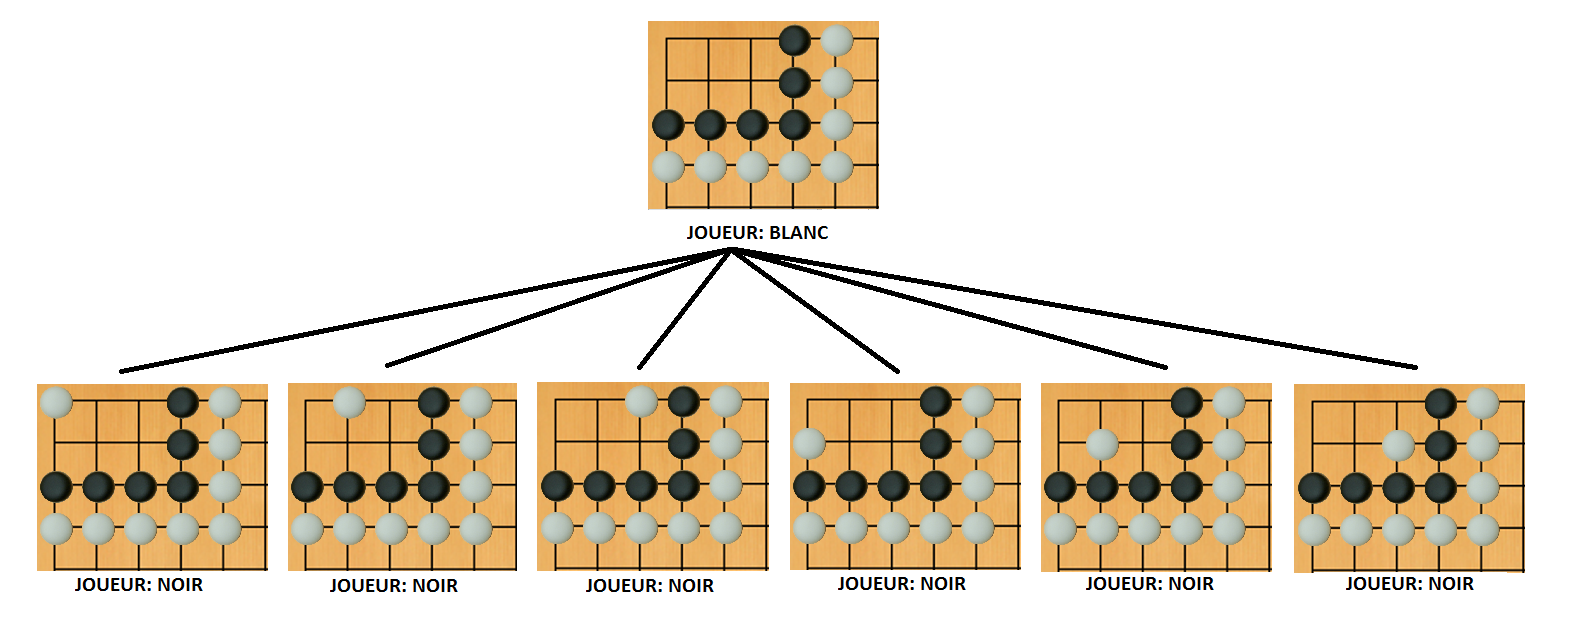
\includegraphics[scale=0.35]{figures/experiments/1.png}
        \caption{Les fils du premier n\oe ud dans le problème du 6 en coin}
        \label{fig:game}
        \end{figure}

        \paragraph{}Notre choix s’est arrêté sur une arborescence à n fils. Chaque nœuds de l’arborescence contient une valeur booléen dont le but est d’indiquer si ce nœud est gagnant.
        L'objet goban permet de connaître l’état de la partie à cet instant dans l’arbre. Chaque fils étant un état du jeu à l’instant T+1 (donc des gobans avec un coup supplémentaire). S’ajoute à cela une valeur, qui vaut blanc ou noir, afin de savoir qui doit jouer si on doit générer des fils à explorer ainsi qu'une variable renseignant le nombre de fils pour l'exploration.

            
    \section{Algorithmes}
        \subsection{Algorithme de définition des fils d'un noeud}
            Pour chaque noeud de l'arbre on calcule tout les coups possibles du joueur et pour chaque coup on crée un goban. On aura de cette manière les gobans des fils qui seront créés successivement à la base de ces premiers.\\
            Le nombre de gobans produit sera intuitivement le nombre d'états vides dans le goban de référence.
            
            \begin{framed}
                \underline{Voici les fonctions de l'algorithme :}
                \begin{itemize}
                    \item \textbf{jouer(Goban, VAL, x, y)}:
                    Soit un Goban et un État la fonction
                    contrôle si par rapport au règles du jeu on peut poser la pierre dans le goban.\\
                    Si la pierre peut être posée alors la placer et renvoyer vraie, sinon renvoyer faux.
                    
                    \item \textbf{rechercheGroupes(g)}:
                    Ajout de l'élément \textit{e} en queue du tableau \textit{t}.
                    
                    \item \textbf{itoc(i, goban)}:
                    Soit un entier et un goban \textit{i} il renvoie les coordonnées (x,y) de l'Etat pointé par \textit{i} dans le goban.
                \end{itemize}
            \end{framed}
            
            \begin{algorithme}
                \caption{définition des gobans fils}
                \textbf{Données :}
                \Type{goban}{Goban},
                \Type{value}{VAL};\\
                \textbf{Résultat :} renvoyer un tableau de gobans\\
                \textbf{Variables :}
                \Type{gob}{Goban},
                \Type{x}{entier},
                \Type{y}{entier},
                \Type{lisGob}{Goban[]},
                \textbf{Début :}\\
                \For{i \textbf{de} 0 \textbf{à} taille(goban)}
                {
                    x$\leftarrow$itoc(i, goban)[0]\\
                    y$\leftarrow$itoc(i, goban)[1]\\
                    gob$\leftarrow$goban\\
                    \If{jouer(gob, value, x, y)}
                    {
                        rechercheGroupes(gob)\\
                        EliminerGroupesAdversaire(value, gob)\\
                        ajoute(gob, listGob)
                    }
                }
                \textbf{renvoyer} listGob
            \end{algorithme}
            
        \subsection{Algorithme récursif du Tsumego}
            \paragraph{}L'algorithme du Tsumego et celui qui va résoudre le problème de vie ou de mort choisie par le joueur. Le principe est de vérifier si un groupe de pierre arrive à s'échapper (voir la partie problèmes plus bas).
            
            \paragraph{}La cible est représentée par une seule pierre appartenant au groupe ciblé. En effet, lorsqu'une pierre appartient à un groupe, celle-ci ne peut être prise si et seulement si le groupe entier est pris. Les données initiale du Tsumego seront donc une pierre, le goban -contenant le problème à résoudre-, l'état relatif à la cible et le joueur courant.
            
            \paragraph{}Si le premier joueur est de la même couleur que la cible alors son but sera de s'échapper. De la manière si le joueur est la couleur opposé il essayera de tuer la cible. 
            Ainsi si le premier joueur gagne alors l'information du noeud sera "vraie", autrement faux.
            
            \paragraph{}Les fils d'un noeud auront comme joueur adverse le joueur père, cela implique que si le fils renvoie l'information "vraie" cela signifiera ainsi qu'il aura survécu, et qu'il est alors nécessaire d'essayer un autre coup, ainsi si ce cas se répète le Tsumego parcourra tout les fils jusqu'à en trouver un qui lui renverra un faux qui signifie qu'il le joueur adverse n'aura pas survécu, donc que le groupe aura été capturé, rimant avec victoire, sinon il continuera à développé l'arbre.
            
            \begin{algorithme}
                \caption{Tsumego}
                \textbf{Données :}
                \Type{A}{Arbre},
                \Type{cible}{Etat};\\
                \textbf{Résultat :} développer \textit{A} pour résoudre le problème de vie ou de mort\\
                \textbf{Variables :}
                \Type{i}{entier},\\
                \textbf{Début :}\\
                \Rem{cas d'arrêt: A est une feuille}\
                \If{nbF(A) = 0}
                {
                    \IfThenElse{couleur(A) = couleur(cible) et enVie(cible,A) = vraie}
                    {
                        A.info = 1
                    }{
                        \IfThenElse{couleur(A)\neq couleur(cible) et enVie(cible,A) = faux}
                        {
                            A.info = 1
                        }{
                            A.info = 0
                        }
                    }
                    \textbf{renvoyer} ;
                }
                
                i$\leftarrow$0\\
                \While{i < nbF(A) et A.info = 0}
                {
                    \IfThenElse{A.joueur = BLANC}
                    {
                        val$\leftarrow$NOIR
                    }{
                        val$\leftarrow$BLANC
                    }
                    \Rem{creation de l'arbre fils}\\
                    A.filsA(GobansFils(A)[i], val)\\
                    \IfThenElse{enVie(cible,A.filsA)}
                    {
                        Tsumego(A.filsA, cible)
                    }{
                        [le coup a tué la cible et l'adversaire est le seul qui peut tuer]\\
                        A.info = 1\\
                        \textbf{renvoyer} ;
                    }
                    
                    \If{A.filsA.info = 0}
                    {
                        A.info = 1\\
                        \textbf{renvoyer} ;
                    }
                    i$\leftarrow$i + 1
                }
            \end{algorithme}
            
    
    
    